\documentclass{beamer}

% balíčky

\usepackage[size=custom, width=120, height=120, scale=1.0, margin=0pt]{beamerposter}
\usepackage{../socstyle}

\usepackage[font={footnotesize}]{caption}
\usepackage[font={footnotesize}]{subcaption}

\renewcommand{\baselinestretch}{1.3}
\renewcommand{\arraystretch}{1.3}


\usepackage{parskip}

\usepackage{tcolorbox}
\tcbuselibrary{breakable}
\definecolor{myblue}{HTML}{172983}
\tcbset{
		colback=myblue!5!white,
		colframe=myblue!75!black,
		fonttitle=\huge\bfseries,
		boxrule=5pt,
		boxsep=24pt,
		parbox=false
}

\usepackage{asymptote}
\def\asydir{asy}

\usepackage{wrapfig}

\usepackage[backend=biber, url=true, sorting=none]{biblatex}
\usepackage{url}
\addbibresource{/home/adam/tex/soc.bib}
\renewcommand*{\bibfont}{\small}

% délky
\newlength{\head}
\setlength{\head}{20cm}

\newlength{\sep}
\setlength{\sep}{1.5cm}

\newlength{\vyska}
\setlength{\vyska}{\paperheight}
\addtolength{\vyska}{-\head}

\newlength{\vyskaA}
\setlength{\vyskaA}{\vyska}
\addtolength{\vyskaA}{-2\sep}

\newlength{\vyskaB}
\setlength{\vyskaB}{\vyska}
\addtolength{\vyskaB}{-\sep}

\newlength{\vyskaC}
\setlength{\vyskaC}{\vyska}
\addtolength{\vyskaC}{-3\sep}

\newlength{\side}
\setlength{\side}{30cm}
\addtolength{\side}{-2\sep}

\newlength{\main}
\setlength{\main}{60cm}
\addtolength{\main}{-2\sep}

\newlength{\newparskip}
\setlength{\newparskip}{12pt}

\setlength{\baselineskip}{82pt}

% témata
\usetheme{Rochester}
\usecolortheme{seahorse}

% posraný zarovnávání
\newlength{\headP}
\setlength{\headP}{\head}
\addtolength{\headP}{-\sep}
\setbeamertemplate{headline}{%
\leavevmode%
  \hbox{%
    \begin{beamercolorbox}[wd=\paperwidth,ht=\headP,dp=0pt]{bg=green}%
    \end{beamercolorbox}%
  }
}
\setbeamertemplate{footline}[frame number]{}
\setbeamertemplate{navigation symbols}{}
\setbeamertemplate{footline}{} 

% asi naprd definice
\title{Mechanika rodin planetek \\ s aplikací na rodinu Eunomia}
\author{Adam Křivka \\ \and doc. Mgr. Miroslav Brož, Ph.\,D.}
\institute{Cyrilometodějské gymnázium a střední odborná škola pedagogická Brno,\\ Lerchova 63, 602 00 Brno}


% ----------


\begin{document}
\begin{frame}
\begin{columns}[t]

\begin{column}{\sep}
\end{column}
\begin{column}{\side}
	\begin{tcolorbox}[title=Úvod\phantom{Úy},height=0.36\vyskaA,parbox=false]
		Planetky jsou nejpočetnější a svým způsobem nejzajímavější skupinou těles ve~sluneční soustavě. První planetka byla objevena v roce 1801, v dnešní době je již známo přes půl milionu planetek.%\\[\newparskip]

		V~hlavním pásu planetek mezi Marsem a~Jupiterem tvoří planetky rodiny --- skupiny vzniklé rozpadem stejného mateřského tělesa, způsobeným srážkou s~jiným tělesem. V~naší práci se soustředíme na početnou rodinu Eunomia, nacházející se ve středním hlavním pásu.%\\[\newparskip]

		Studiem kolizních rodin můžeme zjistit mnoho informací o~vzniku sluneční soustavy a~její dynamické struktuře, např. můžeme podpořit teorii o~\textit{Velkém pozdním bombardování} (angl. \textit{Late Heavy Bombardment})~\cite{broz13}.%\\[\newparskip]
		\begin{figure}[!htb]
			\begin{subfigure}[t]{0.42\textwidth}
			\centering
			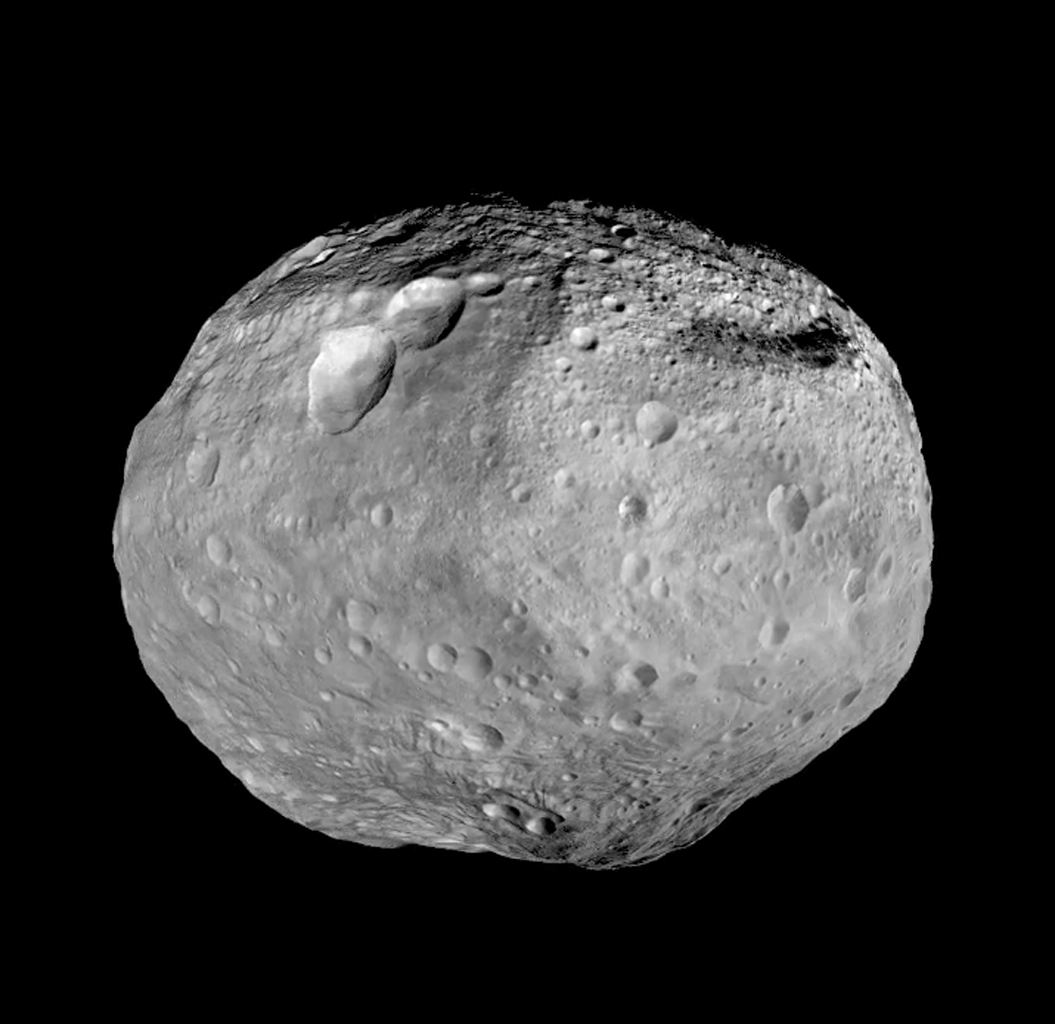
\includegraphics[width=1.0\textwidth]{../obr/vesta.jpg}
			\caption{Planetka (4) Vesta --- druhé největší a~nejhmotnější těleso hlavního pásu planetek.} \label{fig:vesta}
			\end{subfigure}
			\begin{subfigure}[t]{0.56\textwidth}
			\centering
			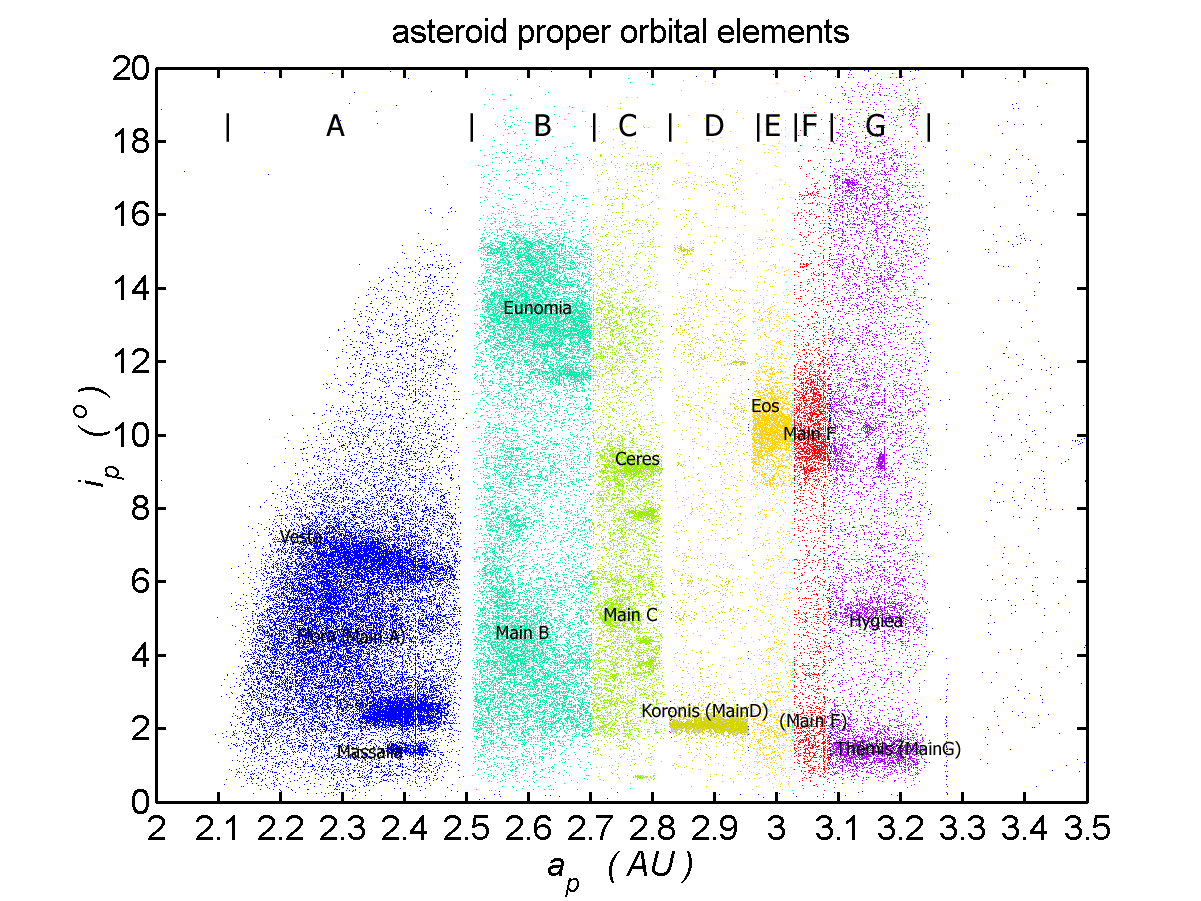
\includegraphics[width=1.0\textwidth]{../obr/mainbelt.png}
			\caption{Hlavní pás planetek v prostoru vlastních elementů dráhy --- vlastní hlavní poloosy $a_{\rm p}$ vlastní sklon $\sin I_{\rm p}$.} \label{fig:belt}
			\end{subfigure}
		\end{figure}
	\end{tcolorbox}

\vspace{\sep}

	\begin{tcolorbox}[title=Metody\phantom{Úy},height=0.64\vyskaA]

		Základním problémem nebeské mechaniky je \textbf{problém $N$ těles} --- vypočítat polohu těles, která na sebe vzájemně gravitačně působí v souladu s \textbf{Newtonovým gravitačním zákonem}.

		{\footnotesize
		\begin{align*} 
			\vec{F}_i = m_i\vec{a}_i &= -\sum_{\substack{j=1 \\ j\neq i}}^N G\frac{m_im_j}{\abs{\vec{r}_i-\vec{r}_j}^3}(\vec{r_i}-\vec{r_j})\,, \qquad{\rm pro}\ i\in\{1,\,2,\,\dots,\,N\ \\
			\vec{a}_i &= -\sum_{\substack{j=1 \\ j\neq i}}^N \frac{Gm_j}{\abs{\vec{r}_i-\vec{r}_j}^3}(\vec{r_i}-\vec{r_j})\,, \qquad{\rm pro}\ i\in\{1,\,2,\,\dots,\,N\ 
		\end{align*}}

K simulaci orbitálního vývoje využíváme \textbf{numerického integrátoru SWIFT}, který počítá s \textbf{Jarkovského jevem}, \textbf{YORP efektem}, \textbf{náhodnými srážkami} i \textbf{chaotickou difuzí}. Zde můžete vidět ilustraci jednodušší integrační metody --- \textbf{Eulerovy metody} --- která je ale pricipielně té naší podobná. 
		\begin{figure}[!htb]
			\centering 
			\begin{subfigure}[b]{0.45\textwidth}
			\centering 
			\asyinclude[width=1.0\textwidth]{../asy/f_euler.asy}
			\end{subfigure}
			\begin{subfigure}[b]{0.45\textwidth}
			\centering 
			\asyinclude[width=1.0\textwidth]{../asy/b_euler.asy}
			\end{subfigure}
			% \caption{Ilustrace dopředné Eulerovy integrační metody pro dvě tělesa. Jsou ukázány první tři iterace. Šedá křivka znázorňuje analytické řešení problému dvou těles.} \label{fig:euler}
		\end{figure}
		Podle pohybu planetky vzhledem ke Slunci můžeme určovat \textbf{elementy dráhy}. Ty se v průběhu času mění působením \textbf{perturbací} (např. gravitační působení ostatních planet), můžeme je tedy přes dlouhé úseky průměrovat na \textbf{střední} a na \textbf{vlastní elementy dráhy}, přičemž druhé z nich jsou nepodléhají žádným periodickým silám.

		\begin{figure}
			\centering
			\begin{subfigure}[b]{0.49\textwidth}
			\centering
			\includegraphics[width=1.0\textwidth]{../obr/atOF}
			\end{subfigure}
			\begin{subfigure}[b]{0.49\textwidth}
			\centering
			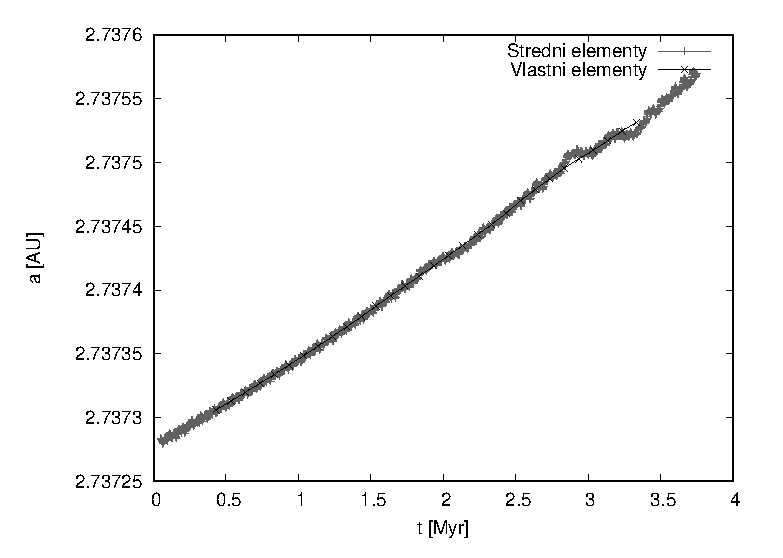
\includegraphics[width=1.0\textwidth]{../obr/atFP}
			\end{subfigure}
			\caption{\ Porovnání oskulační a střední hlavní poloosy (vlevo) a střední a~vlastní hlavní poloosy(vpravo) pro simulaci jedné planetky po dobu $3,76$ miliónů let.}
		\end{figure}
		\begin{tabularx}{\textwidth}{ X X }

\

		K určení členů rodiny používáme \textbf{hierarchickou shlukovací metodu} (HCM) --- v prostoru $(a_{\rm p},\,e_{\rm p},\sin I_{\rm p})$ si zvolíme hraniční vzájemnou \uv{vzdálenost} těles (s jednotkami rychlosti), podle které pak určíme členy.
		{\footnotesize \begin{align*}
			v=na_{\rm p}\sqrt{C_a\left(\frac{\Delta a_{\rm p}}{a_{\rm p}}\right)^2+C_e(\Delta e_{\rm p})^2+C_i(\Delta \sin i_{\rm p})^2}\,,
		\end{align*}}
&
		\begin{figure}
			\centering
			\includegraphics[width=0.5\textwidth]{../obr/Nv}
			\caption{Závislost počtu členů rodiny Eunomia na zvolené hraniční rychlosti $v_{\rm cutoff}$ při použití metody HCM. Počet členů prudce vzroste při přechodu z~rychlosti $43\,{\rm m/s}$ na $44\,{\rm m/s}$, což je způsobené poměrně velkou vzdáleností prvního nejbližšího tělesa od mateřského (15) Eunomia. Dále vzroste prudce při přechodu z~rychlosti $46\,{\rm m/s}$ na $47\,{\rm m/s}$, což je způsobené splynutím s~rodinou Adeona.}
		\end{figure}
		\end{tabularx}

	\end{tcolorbox}

\vspace{\sep}

\end{column}

\begin{column}{2\sep}
\end{column}

\begin{column}{\main}
\begin{tcolorbox}[title=Výsledky\phantom{Úy},height=\vyskaB]
		\begin{figure}
			\centering
			\begin{subfigure}[t]{0.3\textwidth}
				\centering
				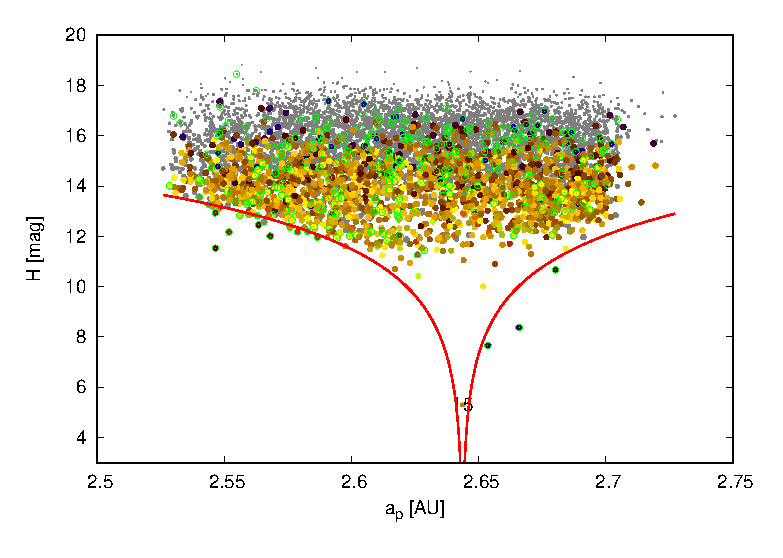
\includegraphics[width=1.0\textwidth]{../obr/aH_wise}
				\caption{Rozdělení pozorované rodiny Eunomia v~rovině vlastní hlavní poloosy $a_{\rm p}$ a~absolutní hvězdné velikosti $H$. Lze pozorovat typický tvar \uv{V}, který je způsobem počátečním rychlostním polem a~Jarkovského jevem, jenž je ještě zesílen vlivem YORPu, což způsobuje zvýšenou koncentraci malých planetek při okrajích rodiny. Pro vyřazení přimísených těles byla použita červená funkce.}
				\label{fig:aH_wise}
			\end{subfigure}
			\begin{subfigure}[t]{0.3\textwidth}
				\centering
				\includegraphics[width=1.0\textwidth]{../obr/pV_pIR}
				\caption{Albeda $p_{\rm V}$ (ve viditelném spektru) a~$p_{\rm IR}$ (v~infračerveném spektru) z~katalogu WISE \cite{nugent15}., barvy neodpovídají reálnému zbarvení. Pro vyřazení přimísených těles touto metodou byly zvoleny hraniční hodnoty $0,05 \leq p_{\rm V} \leq 0,4$.}
				\label{fig:pV_pIR}
			\end{subfigure}
			\begin{subfigure}[t]{0.3\textwidth}
				\centering
				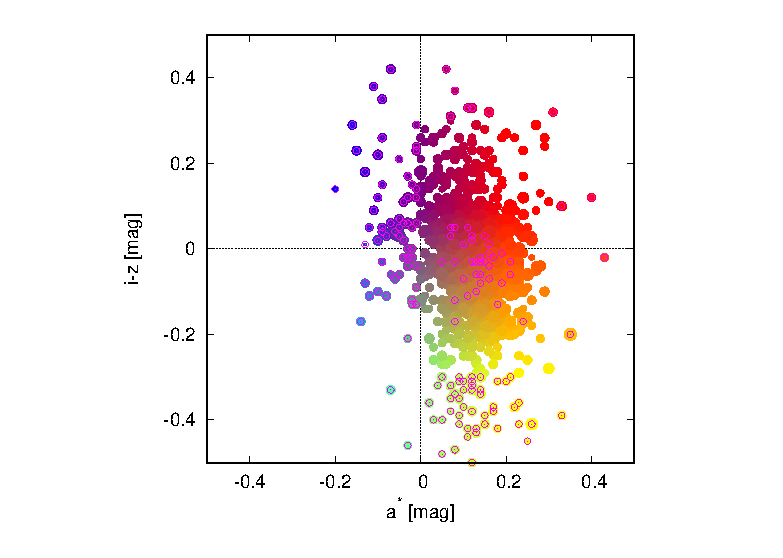
\includegraphics[width=1.0\textwidth]{../obr/astar_iz}
				\caption{Barevné indexy $a^*$ a~$i-z$ z~katalogu Sloan \cite{ivezic01}. Barvy neodpovídají reálnému zbarvení. Pro vyřazení přimísených těles byly zvoleny hraniční hodnoty $0\leq a^* \leq 0,3$ a~$-0,3\leq i-z \leq 0,3$.}
				\label{fig:astar_iz}
			\end{subfigure}
		\end{figure}

		\begin{figure}
			\centering
			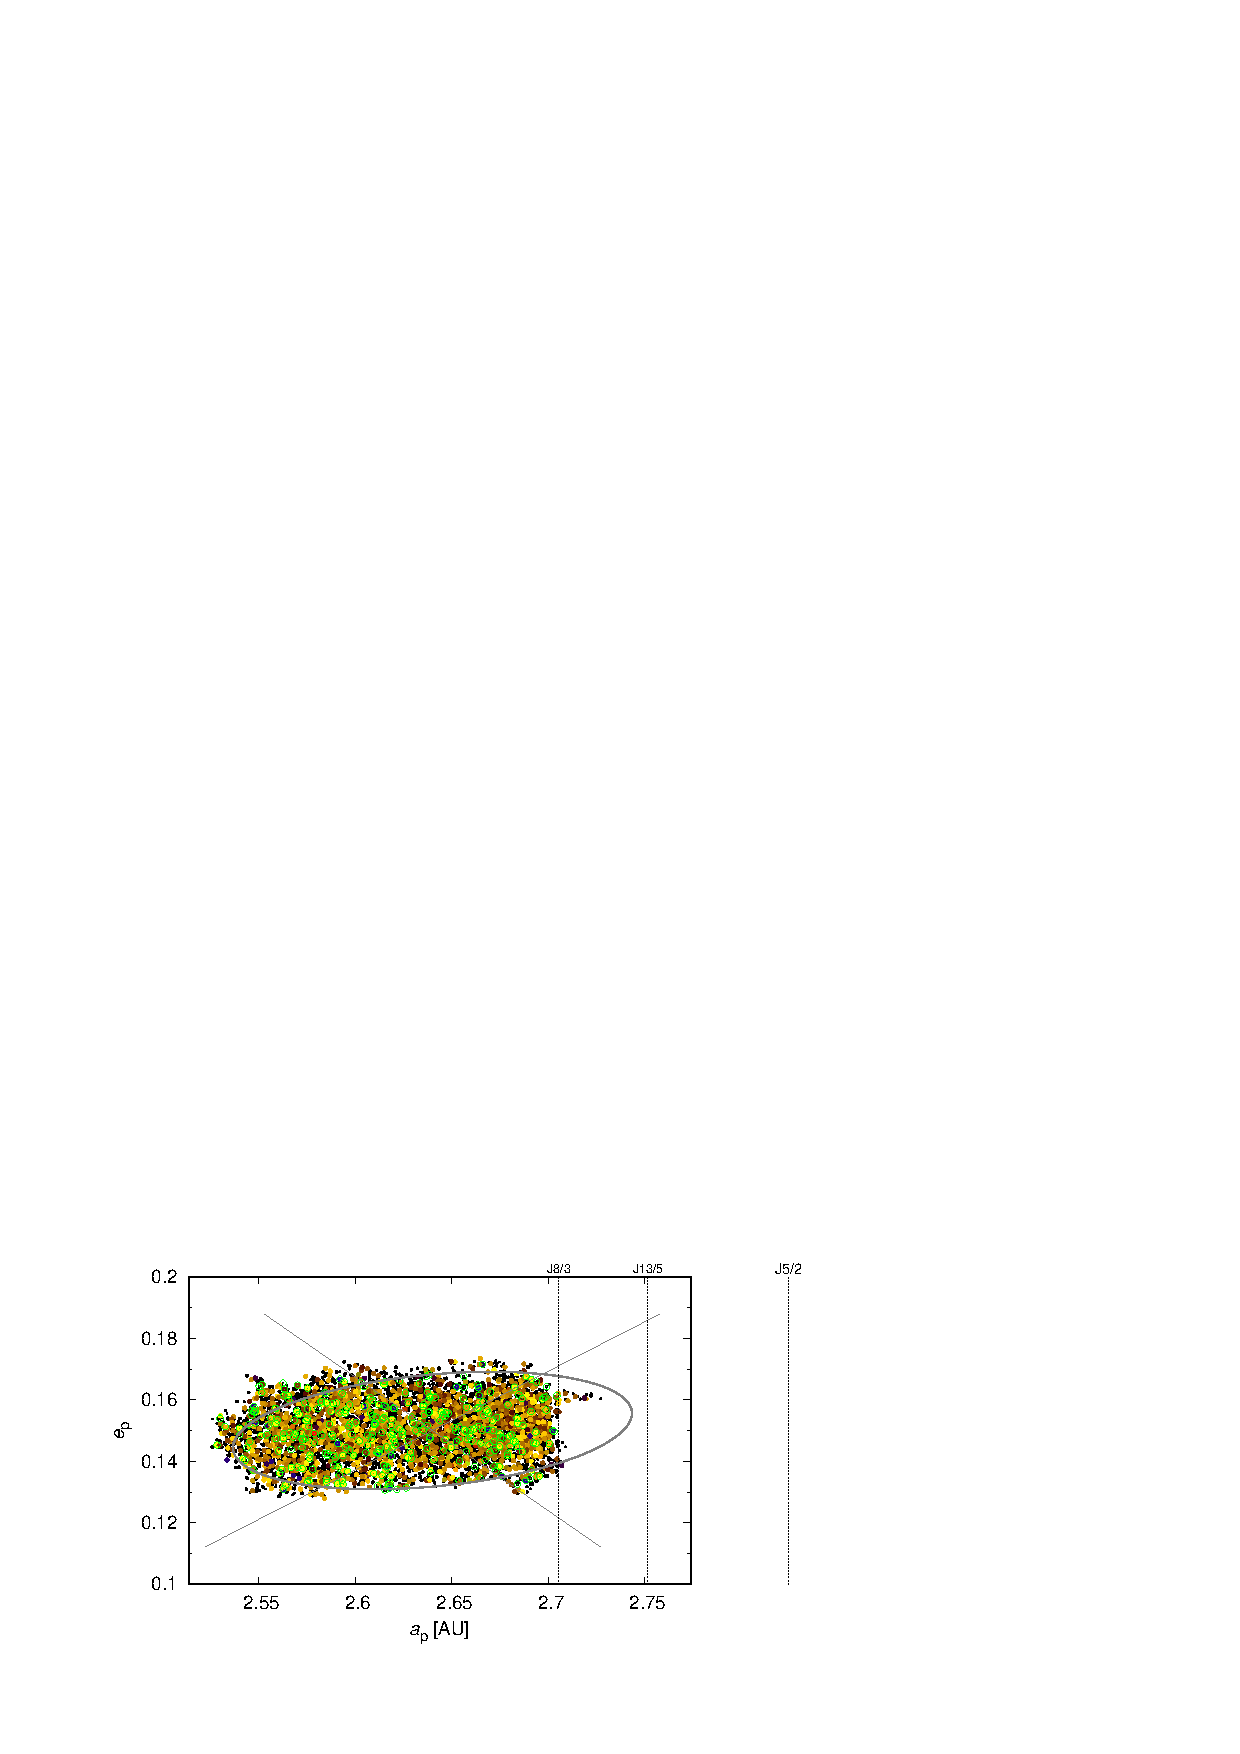
\includegraphics[width=0.49\textwidth]{../obr/ae_wise}
			\includegraphics[width=0.49\textwidth]{../obr/ai_wise}
			\caption{Pozorovaná rodina Eunomia pro hraniční rychlost $v_{\rm cutoff} = 44\,{\rm m/s}$ v~rovině vlastní hlavní poloosy $a_{\rm p}$ a~vlastní excentricity $e_{\rm p}$ (nahoře) a~v~rovině vlastní hlavní poloosy $a_{\rm p}$ a~vlastního sklonu $\sin I_{\rm p}$ (dole). Barevná škála odpovídá albedu $p_{\rm V}$ a~$p_{\rm IR}$ z~katalogu WISE\@. Nápisy J8/3 a~J13/5 označují polohu rezonancí středního pohybu s~Jupiterem. Šedé elipsy a~úsečky (degenerované elipsy) naznačují výpočet Gaussových rovnic pro hodnoty pravé anomálie $f=0^\circ,\,90^\circ,\,180^\circ$ (nahoře) a~součtu $\omega+f=0^\circ,\, 50^\circ,\, 90^\circ$ (dole), kde zvolenou tučnější elipsou je elipsa pro hodnoty $f=90^\circ$ a~$\omega+f=50^\circ$.}
			\label{fig:ae_ai_wise}
		\end{figure}

		\begin{figure}[t]
			\centering
			\begin{subfigure}[t]{0.49\textwidth}
			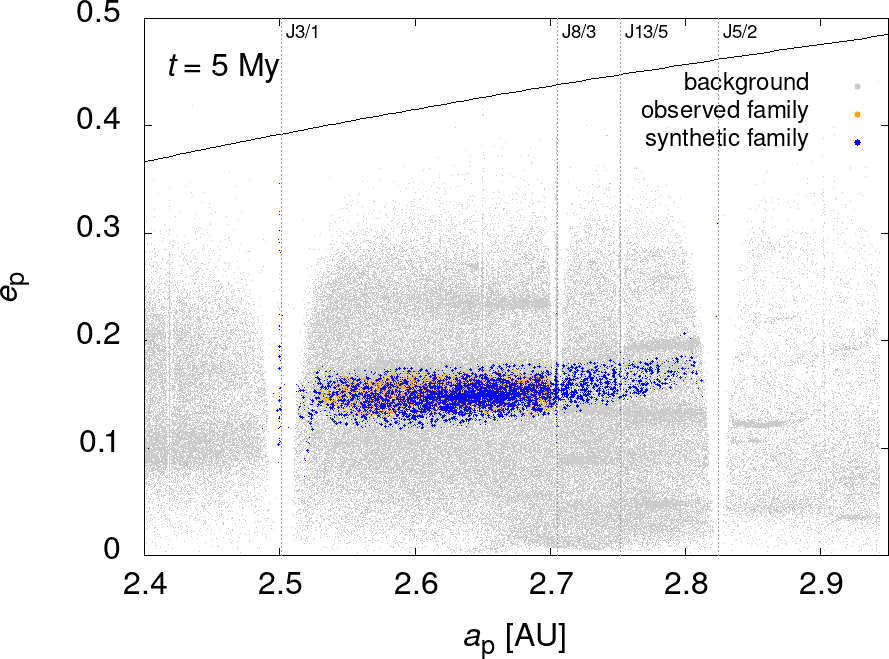
\includegraphics[width=0.49\textwidth]{../obr/ae_5t.png}
			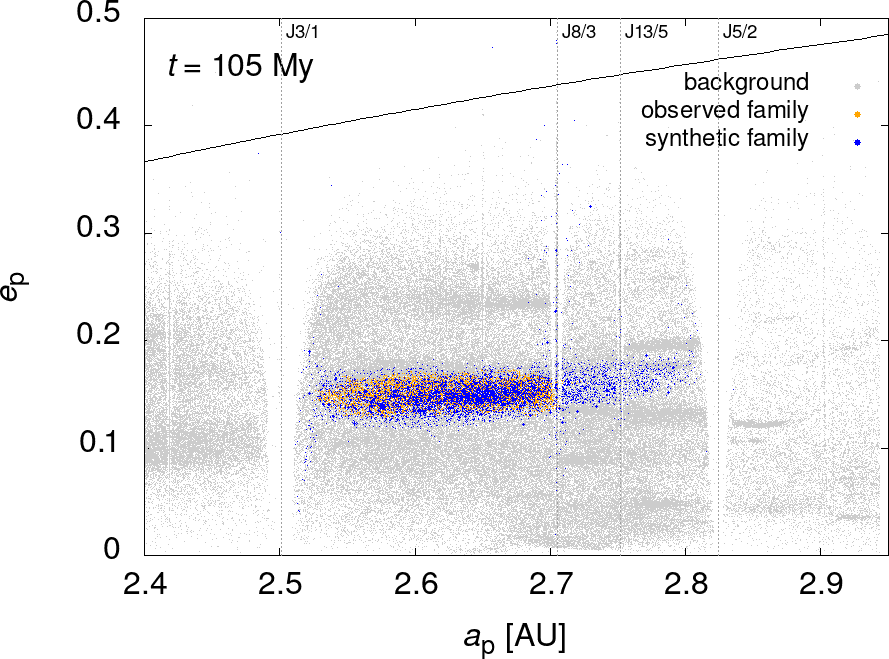
\includegraphics[width=0.49\textwidth]{../obr/ae_105t.png}\\
			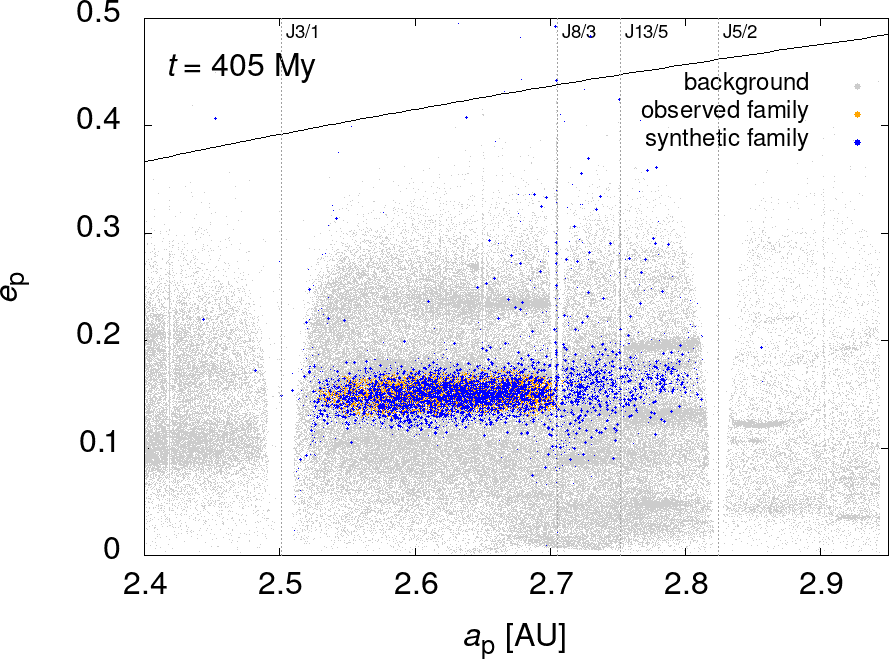
\includegraphics[width=0.49\textwidth]{../obr/ae_405t.png}
			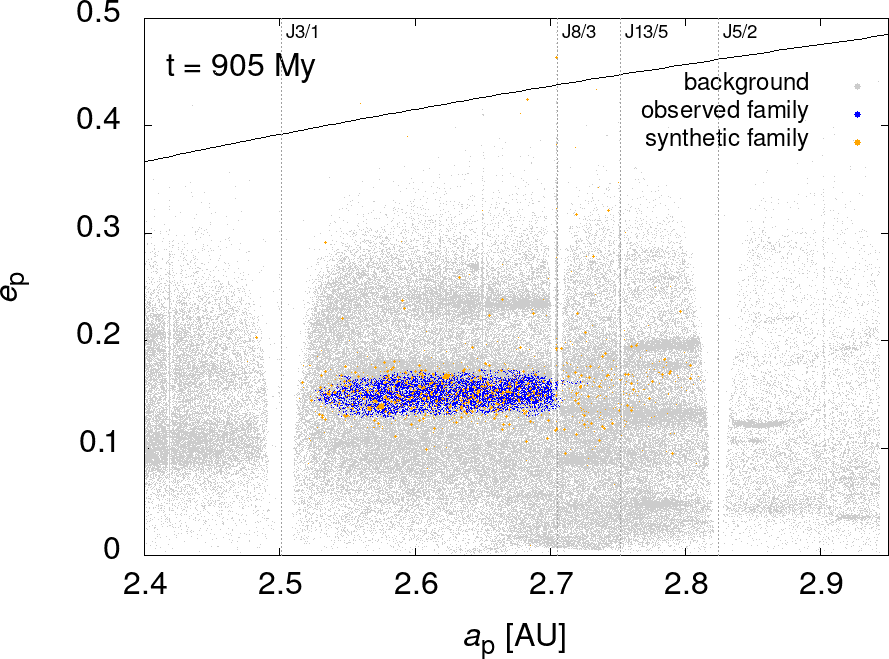
\includegraphics[width=0.49\textwidth]{../obr/ae_905t.png}
			\caption{Výsledky simulace v~prostoru $(a_{\rm p},\,e_{\rm p})$ v~časech postupně $t=5,\,105,\,405,\,905$ miliónů let. Modré body označují simulovanou rodinu, žluté body pozorovanou rodinu identifikovanou HCM a~šedé body pozadí a~jiné okolní rodiny. Jsou také značeny nejvýznamnější rezonance s~Jupiterem J3/1, J8/3, J13/5 a~J5/2. Černá křivka nahoře označuje hranici oblasti, kde je hlavní poloosa a~excentricita tělesa taková, že dráha kříží dráhu Marsu. Podobná hranice existuje i~pro Jupiter, ale ta se nachází mimo tyto grafy (přibližně kolem $e=0,65$). Skripty k~vytvoření těchto grafů můžete nalézt v~příloze \ref{app:fig:ae_sim}.} \label{fig:ae_sim}
			\end{subfigure}
			\begin{subfigure}[t]{0.49\textwidth}
			\centering
			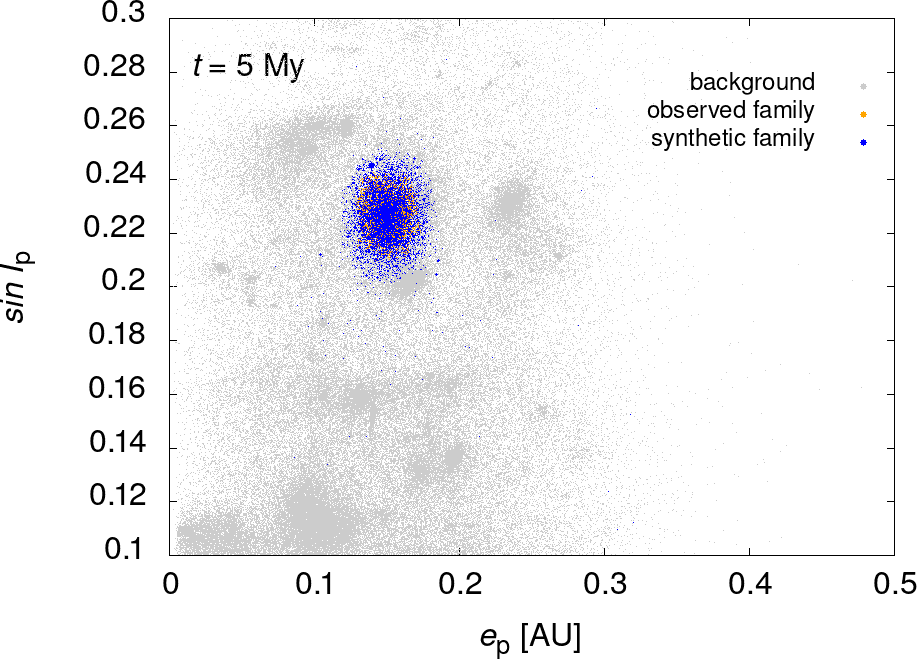
\includegraphics[width=0.49\textwidth]{../obr/ei_5t.png}
			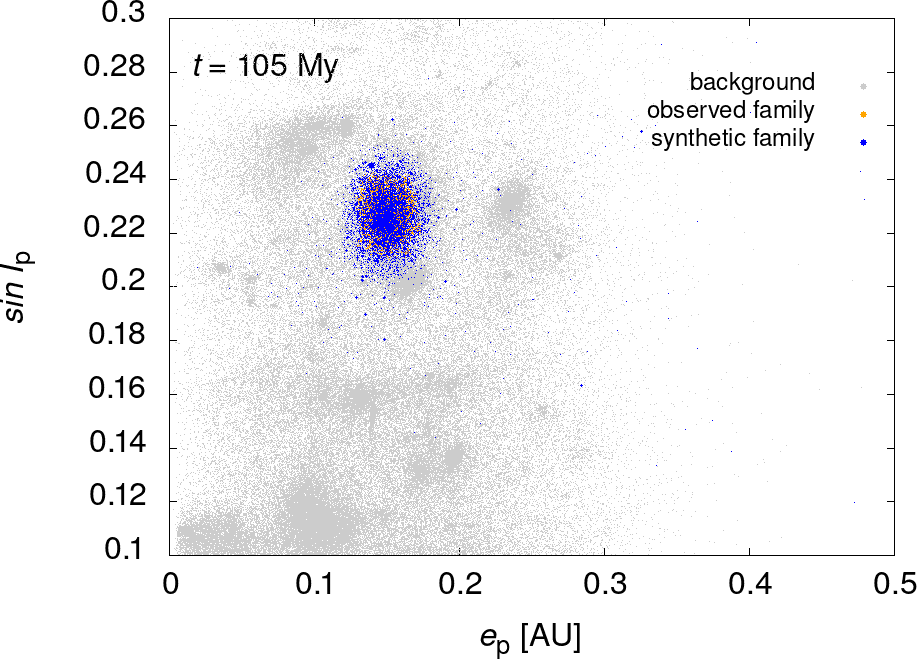
\includegraphics[width=0.49\textwidth]{../obr/ei_105t.png}\\
			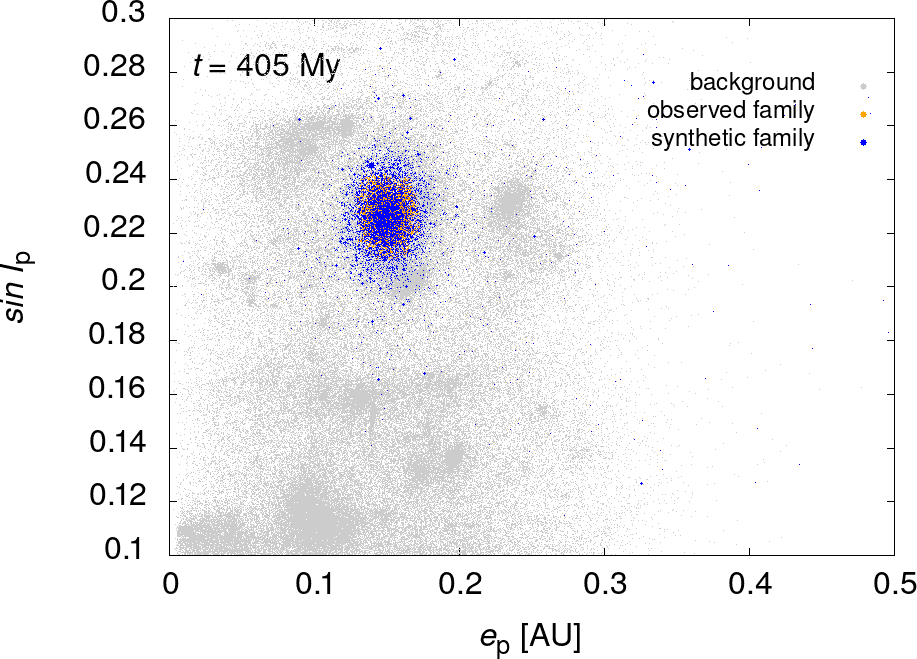
\includegraphics[width=0.49\textwidth]{../obr/ei_405t.png}
			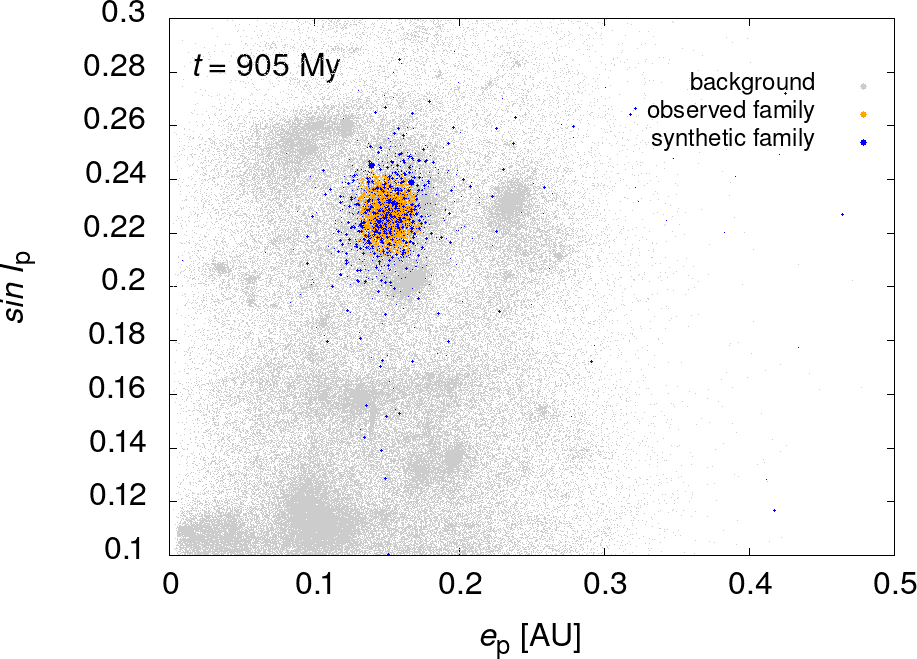
\includegraphics[width=0.49\textwidth]{../obr/ei_905t.png}
			\caption{Výsledky simulace v~prostoru $(e_{\rm p},\,\sin I_{\rm p})$ v~časech postupně $5$, $105$, $405$ a~$905$ miliónů let. Fialový obdélník označuje oblast vybranou pro vzorek populace pozadí.} \label{fig:ei_sim}
			\end{subfigure}
		\end{figure}

		\begin{figure}
			\centering
			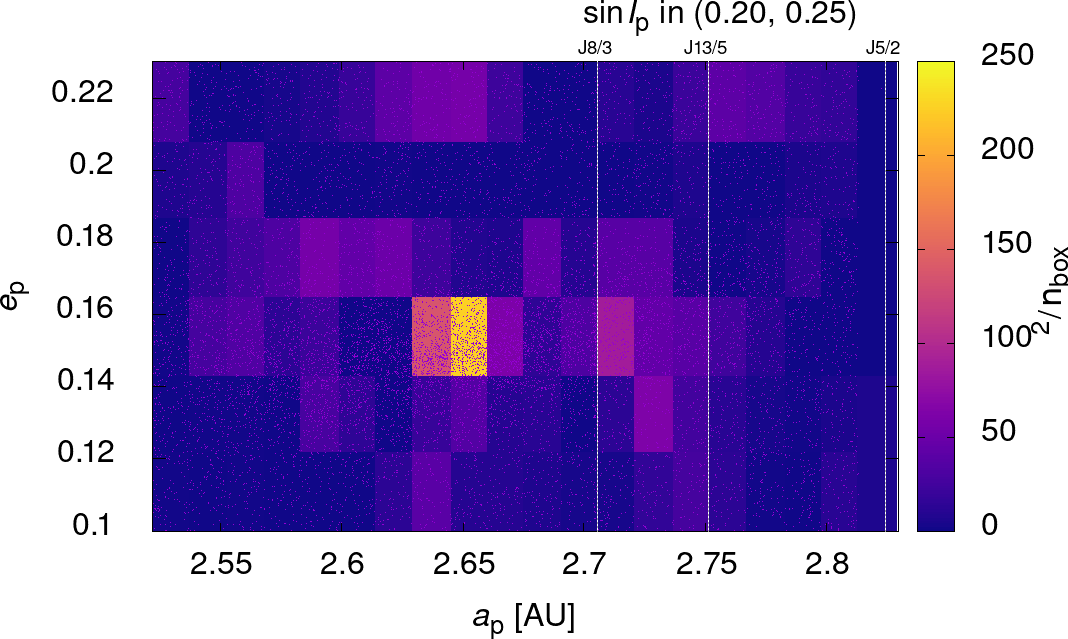
\includegraphics[width=0.49\textwidth]{../obr/ae_chi_0006t.png}
			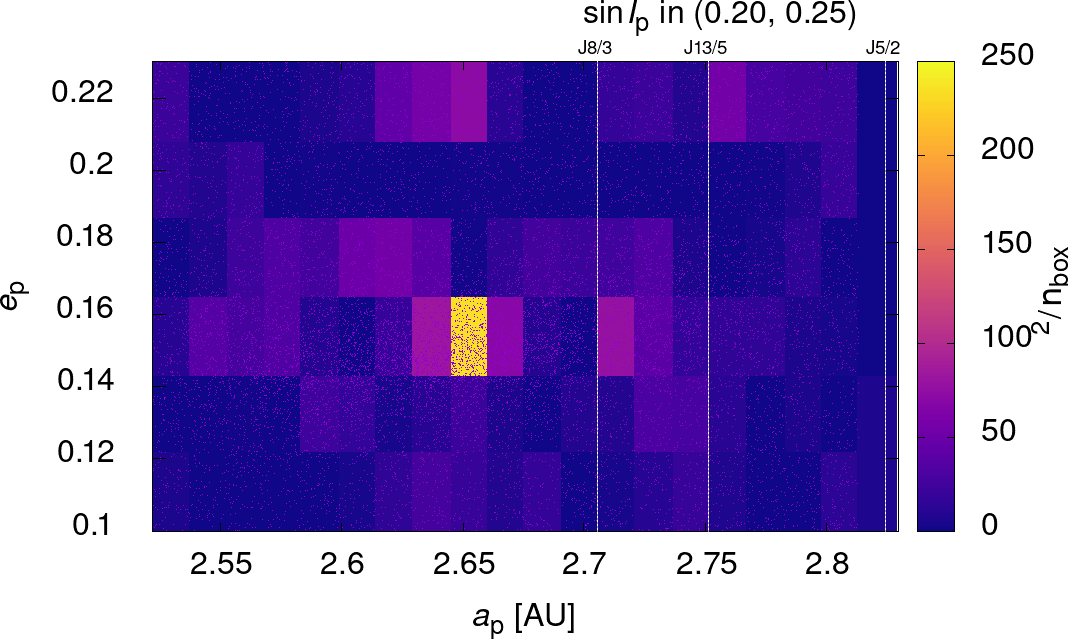
\includegraphics[width=0.49\textwidth]{../obr/ae_chi_0106t.png}\\
			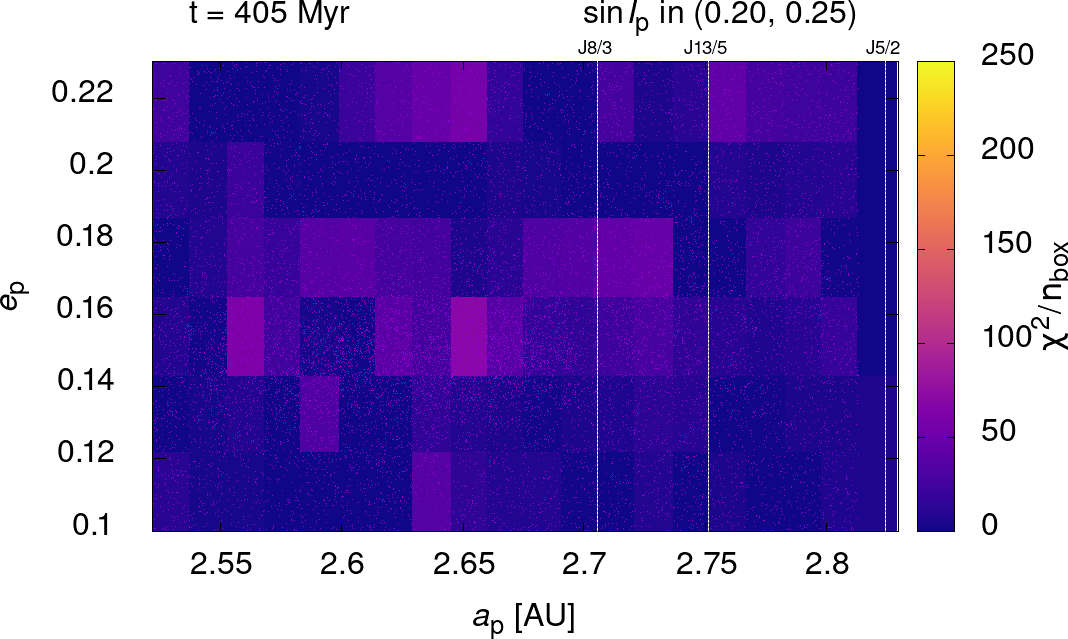
\includegraphics[width=0.49\textwidth]{../obr/ae_chi_0406t.png}
			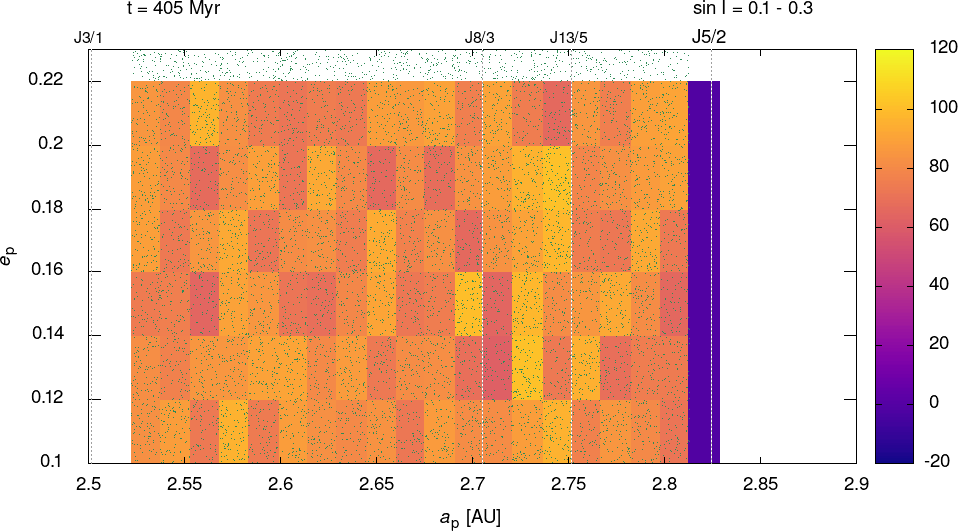
\includegraphics[width=0.49\textwidth]{../obr/ae_chi_emptyt.png}
			\caption{Hodnota chi kvadrátu $\chi^2$ pro každý box v~prostoru $(a,\,e)$. Na prvních třech obrázcích lze vidět rozdělení chi kvadrátu pro $t=5,\,105,\,405$ miliónů let, na posledním obrázku lze vidět rozdělení chi kvadrátu při vygenerování pouze pozadí bez použití částic simulované rodiny. Barevná škála je pro všechny až na poslední obrázek stejná. Zelené tečky označují simulovanou populaci i~s~přidaným pozadím. J8/3, J13/5 a~J5/2 označují rezonance středního pohybu s~Jupiterem.} \label{fig:ae_chi2}
		\end{figure}

\end{tcolorbox}
\vspace{\sep}
\end{column}

\begin{column}{2\sep}
\end{column}

\begin{column}{\side}
\begin{tcolorbox}[title=Závěry\phantom{Úy},height=0.4\vyskaC]
		\begin{figure}
		\centering
		\includegraphics[width=0.49\textwidth]{../obr/ae_scl.png}
		\includegraphics[width=0.49\textwidth]{../obr/ae_obs.png}
		\caption{Graf $(a_{\rm p}, e_{\rm p})$ pro simulovanou (vlevo) a~pozorovanou (vpravo) rodinu Eunomia v~čase $t=455$ miliónů let, kdy byla hodnota $\chi^2$ nejlepší. Tentokrát barevná škála označuje počet těles v~daném boxu. Lze porovnat s~podobným grafem $\chi^2$ --- problémové oblasti jsou přímo v~centru rodiny (simulovaná populace je příliš kompaktní) a~potom v~oblasti $a_{\rm p}\in(2,55\,{\rm AU};\,2,5\,{\rm AU})$ a~$e_{\rm p}\in(0,14;\,0,16)$, kam se naopak částice simulované populace nestihly rozšířit.} \label{fig:ae_obs_scl}
	\end{figure}

\end{tcolorbox}
\vspace{\sep}
\begin{tcolorbox}[title=Budoucí práce\phantom{Úy},height=0.3\vyskaC]
	\begin{figure}
		\centering
		\includegraphics[width=0.7\textwidth]{../obr/chi2.eps}
		\caption{Závislost redukovaného chí kvadrátu $\chi^2/n_{\rm box}$ na čase $t$. Lze vidět, že se jeho hodnota snižuje, tudíž můžeme předpokládat, že bychom delší integrací dostali nižší hodnoty, případně bychom mohli určit interval stáří rodiny Eunomia.} \label{fig:chi2}
	\end{figure}
\end{tcolorbox}
\vspace{\sep}
\begin{tcolorbox}[title=Reference\phantom{Úy},height=0.3\vyskaC]
		\printbibliography
\end{tcolorbox}
\end{column}

\begin{column}{\sep}
\end{column}

\end{columns}
\end{frame}
\end{document}
